\documentclass[conference]{IEEEtran}
\IEEEoverridecommandlockouts
\usepackage{cite}
\usepackage{amsmath,amssymb,amsfonts}
\usepackage{newtxtext,newtxmath}
\usepackage{graphicx}
\usepackage{booktabs}
\usepackage{textcomp}
\usepackage{xcolor}
\usepackage[hyphens]{url}
\def\BibTeX{{\rm B\kern-.05em{\sc i\kern-.025em b}\kern-.08em T\kern-.1667em\lower.7ex\hbox{E}\kern-.125emX}}
\begin{document}

\title{Measuring the Attacker-Side Fingerprintability of a Multi-Protocol LLM-Backed Honeypot:\\Protocol Conformance and Timing Side Channels}

\author{
\IEEEauthorblockN{Dharshini Sanapureddy\textsuperscript{1}, Naga Jyohi Darisa\textsuperscript{2}, Sadhwika Tulasi\textsuperscript{3}, Rohith Reddy T\textsuperscript{4}, Radhika G\textsuperscript{5}}
\IEEEauthorblockA{\textit{Department of Computer Science and Engineering}\\
\textit{Amrita School of Computing, Coimbatore}\\
\textit{Amrita Vishwa Vidyapeetham, India}\\
cb.sc.u4cse24746@cb.students.amrita.edu\textsuperscript{1}, cb.sc.u4cse24214@cb.students.amrita.edu\textsuperscript{2},\\
cb.sc.u4cse24054@cb.students.amrita.edu\textsuperscript{3}, cb.sc.u4cse24551@cb.students.amrita.edu\textsuperscript{4}, g\_radhika@cb.amrita.edu\textsuperscript{5}}
}

\maketitle

\begin{abstract}
Large language models let a honeypot answer commands it was never scripted for, but every generated answer arrives late and some arrive wrong. This paper measures how easily a remote attacker can tell a three-tier LLM-backed honeypot (static table, response cache, hosted LLM) from the real services it imitates, across three protocols: an SSH shell compared with OpenSSH, an Ethereum JSON-RPC endpoint compared with a reference node, and a CI server compared with Jenkins. We define 28 black-box conformance probes and find that 21 of them distinguish the decoy deterministically, including an unevaluated shell arithmetic expression, acceptance of arbitrary credentials, and a rejected JSON-RPC batch. On timing, a single-observation latency detector separates the LLM tier from the real service with AUC 1.000 in every protocol (median 929\,ms against 1.2\,ms for a novel SSH command); the static and cache tiers are also separable (AUC 1.000) because the decoy's extra HTTP hop makes a scripted reply 9$\times$ slower than OpenSSH, although that gap is small enough for Internet jitter to mask. Replaying a 2,500-payload corpus of real-world attack strings through the engine shows that none of it is served by the static tier: 100\% reaches the model, at a median of 1,363\,ms and a p95 of 8,567\,ms. Because attack payloads are structurally unique, a cache warmed on half of the corpus serves 0\% of the other half with exact keys and 0.2\% with normalized keys. The identity and protocol defects are cheap to remove and we list the fixes; the timing gap is not closed by caching and must be addressed by faster generation or by routing more traffic to deterministic tiers.
\end{abstract}

\begin{IEEEkeywords}
honeypot, cyber deception, large language models, fingerprinting, timing side channel, protocol conformance, SSH, JSON-RPC
\end{IEEEkeywords}

\section{Introduction}
A honeypot is only useful while the attacker believes it. Classical low- and medium-interaction honeypots are believed for a short time: their canned responses, default banners and missing protocol features are fingerprintable at Internet scale~\cite{ref3,ref4}, and network-level timing anomalies were reported as early as 2006~\cite{ref2}. Large language models (LLMs) appear to remove the first limitation. A model that generates a plausible shell listing, SQL error or JSON-RPC result for any input has no canned-response boundary to probe~\cite{ref5,ref6,ref7,ref8}. A recent systematization of LLM honeypots nevertheless lists response timing as ``a critical and unresolved challenge''~\cite{ref9}, and benchmarking studies report that LLM backends differ from one another by an order of magnitude in latency~\cite{ref10,ref11}. What none of this work reports is the quantity that matters to an attacker: how separable the honeypot is from the genuine service it claims to be, under probes the attacker can send from outside.

This paper measures that quantity for a deployed multi-protocol honeypot whose response engine has three tiers, a static command table, a Redis cache and a hosted LLM (Fig.~\ref{fig:pipeline}). We probe each decoy and its real counterpart identically and ask three questions. Which deterministic probes reveal the decoy regardless of timing? How well does response latency alone reveal it, per tier? And how much of a realistic attack corpus actually reaches the slow tier, so that caching could in principle hide it? The contributions are:
\begin{enumerate}
\item A conformance probe set of 28 black-box tests across SSH, JSON-RPC and HTTP, with reference behavior measured on OpenSSH, an Ethereum client and Jenkins (Section~\ref{sec:method}); 21 probes distinguish the decoy (Section~\ref{sec:res-conf}).
\item A per-tier timing analysis with 30 trials per probe class, reported as latency distributions and the AUC of a single-observation detector (Section~\ref{sec:res-time}).
\item A tier-exposure measurement over a 2,500-payload corpus of real-world attack strings, and an analysis of exact-match versus normalized cache keys that bounds what caching can hide (Sections~\ref{sec:res-corpus} and \ref{sec:res-cache}).
\item A ranking of mitigations by implementation cost and by which of the three fingerprint classes they remove (Section~\ref{sec:discussion}).
\end{enumerate}

\section{Related Work}
Provos's virtual honeypot framework established emulated services as sensors~\cite{ref1}. Defibaugh-Chavez et al.\ showed that emulated services and virtual environments can be recognized from network-level behavior, including response times to simple requests~\cite{ref2}. Vetterl and Clayton fingerprinted low- and medium-interaction honeypots at Internet scale by finding protocol responses in which the honeypot implementation deviates from the software it imitates~\cite{ref3}, and Morishita et al.\ measured how many deployed honeypots reveal themselves through default configurations~\cite{ref4}. Our conformance probes follow the same logic, applied to a system whose responses are partly generated rather than scripted.

LLM honeypots began with shelLM~\cite{ref5}, which showed that a model can sustain a believable Linux shell, and with Ragsdale and Boppana's low-risk design that curates model inputs~\cite{ref6}. Weber et al.\ proposed a unified evaluation of response quality~\cite{ref7}; LLMHoney reports mean latencies near three seconds for hosted models~\cite{ref8}; Magazov et al.\ benchmark eleven backends and find that a classifier can identify the backend from a single response, and separately route commands to different models by attack phase to trade fidelity against latency~\cite{ref10,ref11}. The SoK by Bridges et al.\ organizes detection vectors against LLM simulation capabilities and identifies timing as open~\cite{ref9}. These studies measure the honeypot's own latency; we measure its distinguishability from the real service, which requires probing both under the same client and conditions, and we do so for three protocols rather than SSH alone.

\section{System Under Test and Threat Model}
\label{sec:system}
\begin{figure}[!t]
\centering
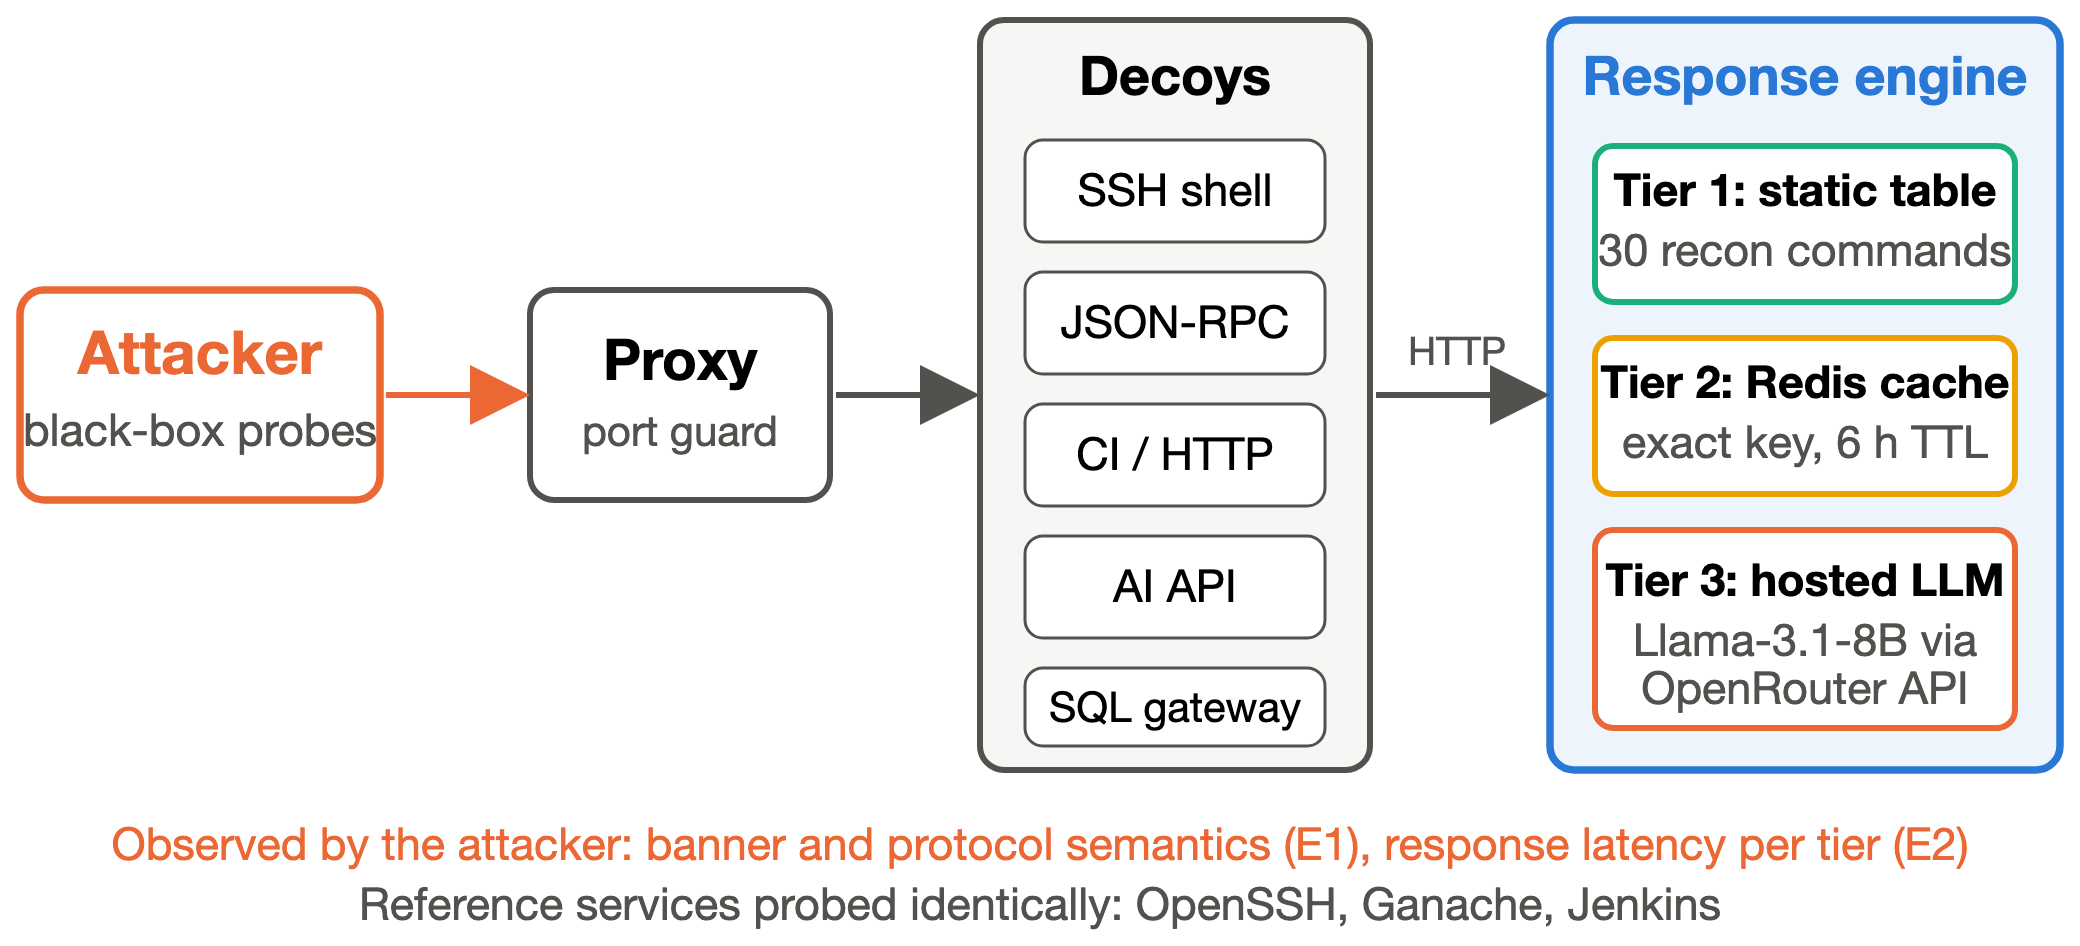
\includegraphics[width=\columnwidth]{figures/diag_pipeline.png}
\caption{The honeypot under test. Five decoys sit behind a port-guarding proxy and obtain their answers from a three-tier response engine. The attacker observes only protocol behavior and timing; the same probes are sent to reference implementations of each service.}
\label{fig:pipeline}
\end{figure}

\subsection{Honeypot}
The system is a containerized deception platform built by the authors; the evaluation treats it as an opaque target, and the harness can be pointed at any honeypot that exposes the same protocols. A TCP proxy exposes five ports and forwards each to a decoy: an SSH shell built on the \texttt{asyncssh} library~\cite{ref12}, an Ethereum JSON-RPC endpoint~\cite{ref13,ref14}, a Jenkins-like CI server, an internal AI inference API, and an HTTP gateway to a seeded PostgreSQL database. Each decoy logs the interaction and asks a shared response engine for the reply. The engine answers in three tiers. Tier~1 is a static table of 30 reconnaissance commands (\texttt{whoami}, \texttt{uname -a}, \texttt{cat /etc/passwd}, \ldots) plus prefix rules for \texttt{cd}, \texttt{sudo}, \texttt{echo} and file-creation commands; it applies to the SSH decoy only. Tier~2 is a Redis cache keyed on the MD5 of the command and the last two commands of the session, with a six-hour TTL. Tier~3 is a hosted model (Llama-3.1-8B-Instruct through the OpenRouter API) with a per-service system prompt and a 60-token response limit. A decoy therefore answers from tier~1 in microseconds plus one HTTP hop, from tier~2 in one Redis lookup plus the hop, and from tier~3 after a remote inference call.

\subsection{Attacker}
The attacker is remote, has no foothold, and interacts only through the exposed ports as an ordinary client would. It may compare what it observes with the behavior of the software the decoy claims to be, and it may time its own requests. It sends a handful of requests per host, so a detector that needs a single observation is more useful to it than one that needs a distribution. We do not consider attackers that have compromised the honeypot host or that observe network traffic elsewhere.

\subsection{Reference services}
Each decoy is compared with a real implementation run in the same Docker environment on the same machine: OpenSSH 10.3 (banner \texttt{SSH-2.0-OpenSSH\_10.3}, password authentication enabled), Ganache 7.9.2~\cite{ref16} as the Ethereum node (banner \texttt{Ganache/v7.9.2/EthereumJS TestRPC/v7.9.2/ethereum-js}), and Jenkins 2.541.3 (Jetty(12.1.5)). The AI API and SQL gateway have no canonical counterpart, since they imitate internal services rather than a named product, and are excluded from the pairwise comparison; their payload classes still appear in the corpus experiment.

\section{Method}
\label{sec:method}
All measurements are made by one harness (\texttt{benchmark\_fingerprint.py}) from the host, through the proxy for decoys and directly for reference services, over the loopback interface, in a single run of 38 minutes.

\textbf{E1, conformance.} For each protocol a fixed list of black-box probes is sent to decoy and reference and the observable answer is recorded: for SSH the version banner, host-key type, cipher negotiated by the same client, whether random credentials are accepted, whether an \texttt{exec} request is honored, and the output of six shell commands chosen to exercise arithmetic expansion, compound commands, error message format and state (\texttt{cd} then \texttt{pwd}); for JSON-RPC the client version, chain id, the error object for an unknown method, the response to a malformed body, id echoing, batch requests, missing parameters, block-number monotonicity and the field count of a block object; for the CI server status codes and headers for the root, \texttt{/api/json}, an unknown path, \texttt{/login}, \texttt{HEAD}, \texttt{/robots.txt} and a build trigger. A probe is \emph{distinguishing} when the two answers differ.

\textbf{E2, timing.} For each protocol and tier, 30 trials measure the wall-clock time from sending a request to receiving the complete reply, for the decoy and for the reference under the same client code. SSH classes are connect-plus-authenticate, a static-tier recon command, a novel command with a random suffix (LLM tier), the same novel command repeated (cache tier), and a five-command reconnaissance session. JSON-RPC classes are a method in the decoy's static table, a novel \texttt{eth\_getStorageAt} call (LLM tier) and its repeat (cache tier). CI classes are an unknown path (the framework's static 404), \texttt{GET /api/json} (generated once, then served from the cache because its key is constant) and a build \texttt{POST} with a random parameter (LLM tier). Distinguishability is reported as the AUC of a threshold detector, $\Pr[t_{\mathrm{decoy}} > t_{\mathrm{real}}]$, which equals the Mann--Whitney statistic~\cite{ref15}; an AUC near 0 means the decoy is reliably \emph{faster}. Where the two distributions overlap we also report the accuracy of the best single threshold in either direction, the detector an attacker with one observation would use.

\textbf{E3, tier exposure.} The platform's evaluation corpus of 2,500 real-world attack payloads (SQL injection, command injection, XXE, prompt injection, Ethereum RPC abuse, Jenkins exploitation; each tagged with a unique nonce) is replayed through the response engine with 8 concurrent clients. Before each request the harness decides which tier will answer by applying the static rules and checking the cache for the exact key; the reply latency is recorded per tier. A second pass over a 300-payload sample measures cache-tier latency once every key is warm.

\textbf{E4, cache reuse.} The corpus is split in half. Exact keys and normalized keys (nonce and comment suffixes removed, whitespace collapsed, long hexadecimal and numeric literals replaced by placeholders) from the first half are used to count how many payloads of the second half would hit the cache. This bounds the fraction of \emph{new} attacker traffic that a warmed cache can serve without reaching the model.

\section{Results}
\label{sec:results}

\subsection{Conformance}
\label{sec:res-conf}
Table~\ref{tab:conf} lists every probe. 21 of 28 distinguish the decoy: 7/11 for SSH, 7/9 for JSON-RPC and 7/8 for the CI server. Three classes of defect appear. The first is implementation identity: the SSH banner names the \texttt{asyncssh} library, the RPC client version is generated by the model and varied between runs (\texttt{Ethereum/Clique/2.0} in one, \texttt{Istanbul} in another), neither in the form a real client emits, and the CI server reports \texttt{uvicorn} where Jenkins reports Jetty and adds \texttt{X-Jenkins} headers. The second is protocol coverage: the decoy accepts any credentials, does not honor \texttt{exec} requests, rejects JSON-RPC batches and malformed bodies with HTTP 500, and answers \texttt{HEAD}, \texttt{/login} and \texttt{/robots.txt} with 404. The third is fast-path semantics: tier~1 returns \texttt{\$((7*6))} unevaluated, treats \texttt{cd /tmp; pwd} as a directory named \texttt{/tmp; pwd}, and hands a compound command to the model, which reports it as not found. The model itself did well where it was reached: its error message for a missing file matched the real shell byte for byte.

\begin{table*}[!t]
\caption{E1: black-box conformance probes, decoy versus reference implementation}
\label{tab:conf}
\centering
\footnotesize
\renewcommand{\arraystretch}{1.12}
\begin{tabular}{@{}p{0.25\textwidth}p{0.29\textwidth}p{0.31\textwidth}c@{}}
\toprule
Probe & Decoy & Reference & Distinguishes \\
\midrule

\multicolumn{4}{@{}l}{\textit{SSH} (7 of 11 probes distinguish)} \\
Version banner & AsyncSSH 2.23.1 & OpenSSH 10.3 & yes \\
Host-key type & ssh-rsa & ssh-rsa & no \\
Cipher negotiated & chacha20-poly1305 & chacha20-poly1305 & no \\
Random credentials accepted & yes & no & yes \\
\texttt{exec} request honored & no & yes & yes \\
\texttt{echo \$((7*6))} & \$((7*6)) & 42 & yes \\
\texttt{cat} missing file & No such file or directory & No such file or directory & no \\
Unknown command & ``command not foun'' (truncated) & ``-bash: \ldots: command not found'' & yes \\
\texttt{cd /tmp; pwd} & (empty) & /tmp & yes \\
\texttt{hostname; uname -n} & command not found & same name twice & yes \\
\texttt{echo 'a  b'} & a  b & a  b & no \\
\midrule
\multicolumn{4}{@{}l}{\textit{JSON-RPC} (7 of 9 probes distinguish)} \\
\texttt{web3\_clientVersion} & Istanbul & Ganache/v7.9.2/... & yes \\
\texttt{eth\_chainId} & 1 & 0x539 & yes \\
Unknown method & error -32601 & error -32700 & yes \\
Malformed body & HTTP 500 & HTTP 400 & yes \\
String id echoed & 'abc' & 'abc' & no \\
Batch request & HTTP 500 & HTTP 200, 2 results & yes \\
\texttt{eth\_getBalance}, no params & result, no error & error -32700 & yes \\
\texttt{eth\_blockNumber} twice & constant & constant & no \\
\texttt{eth\_getBlockByNumber} & result, no error & 23 fields & yes \\
\midrule
\multicolumn{4}{@{}l}{\textit{CI/HTTP} (7 of 8 probes distinguish)} \\
\texttt{GET /} & HTTP 404, uvicorn & HTTP 200, Jetty(12.1.5), X-Jenkins & yes \\
\texttt{GET /api/json} & JSON key result only & JSON keys \_class, assignedLabels, \ldots & yes \\
\texttt{GET} unknown path & HTTP 404, uvicorn & HTTP 404, Jetty(12.1.5) & yes \\
\texttt{GET /login} & HTTP 404, uvicorn & HTTP 200, Jetty(12.1.5) & yes \\
\texttt{HEAD /} & HTTP 404, uvicorn & HTTP 200, Jetty(12.1.5) & yes \\
\texttt{GET /robots.txt} & HTTP 404 & HTTP 200 & yes \\
\texttt{POST} build trigger & HTTP 200, uvicorn & HTTP 403, Jetty(12.1.5) & yes \\
\texttt{GET /api/json} repeated & identical & identical & no \\
\bottomrule
\end{tabular}
\end{table*}

\subsection{Timing}
\label{sec:res-time}
Table~\ref{tab:timing} and Fig.~\ref{fig:latency} report E2. The LLM tier is separable in every protocol: a novel SSH command takes a median of 929\,ms on the decoy (p95 7,349\,ms, minimum 558\,ms) against 1.2\,ms on OpenSSH, for an AUC of 1.000; a novel RPC call takes 1,412\,ms against 7.6\,ms (AUC 1.000); and a build \texttt{POST} to the CI decoy takes 3,495\,ms against 8.3\,ms on Jenkins (AUC 1.000). The slowest reference reply in each class is faster than the fastest model reply, so any threshold between them classifies every trial correctly. Repeating a command inside the same SSH session does not help the decoy: the cache key includes the previous two commands, so the repeat is a fresh model call (median 1,385\,ms).

The fast tiers also leak, by a smaller margin. A static-tier SSH command answers in 11.8\,ms on the decoy against 1.3\,ms on OpenSSH (AUC 1.000), the difference being the HTTP hop from the decoy to the engine; the cache tier behaves the same way (8.6\,ms, AUC 1.000), and a five-command reconnaissance session served entirely from tier~1 takes 60\,ms against 6\,ms. For JSON-RPC a method in the decoy's static table takes 23.5\,ms against 3.0\,ms (AUC 1.000), and a cached CI status page 28\,ms against 3.8\,ms. Connect-plus-authenticate is the weakest signal: 35\,ms against 33\,ms (AUC 0.924, best threshold 87\% accurate), because the decoy posts the captured credentials to its backend before replying. One probe leaks in the opposite direction: an unknown path on the CI decoy is answered by the framework's 404 handler in 7.3\,ms, faster than Jenkins renders its error page (15.5\,ms, AUC 0.000). All fast-tier gaps are of the order of ten milliseconds, one local round trip, and would be masked by the variance an attacker sees across the Internet; they are laboratory fingerprints. The LLM-tier gap is three orders of magnitude and survives any network.

\begin{table}[!t]
\caption{E2: response latency, decoy vs.\ reference (30 trials per class; ms)}
\label{tab:timing}
\centering
\scriptsize
\renewcommand{\arraystretch}{1.15}
\setlength{\tabcolsep}{3.5pt}
\begin{tabular}{@{}llrrrrr@{}}
\toprule
& & \multicolumn{2}{c}{Decoy} & \multicolumn{2}{c}{Reference} & \\
\cmidrule(lr){3-4}\cmidrule(lr){5-6}
Service & Probe class & med. & p95 & med. & p95 & AUC \\
\midrule
SSH & connect + authenticate & 35.3 & 43 & 33.0 & 35.1 & 0.924 \\
SSH & recon command (static) & 11.8 & 14 & 1.3 & 2.8 & 1.000 \\
SSH & repeated command (cache) & 8.6 & 9 & 1.2 & 1.7 & 1.000 \\
SSH & novel command (LLM) & 928.9 & 7,349 & 1.2 & 1.5 & 1.000 \\
SSH & 5-command recon session & 60.5 & 63 & 6.4 & 7.8 & 1.000 \\
JSON-RPC & known method (static) & 23.5 & 27 & 3.0 & 3.8 & 1.000 \\
JSON-RPC & repeated call (cache) & 44.6 & 49 & 4.0 & 4.7 & 1.000 \\
JSON-RPC & novel call (LLM) & 1,411.5 & 13,015 & 7.6 & 10.8 & 1.000 \\
CI/HTTP & unknown path (404) & 7.3 & 8 & 15.5 & 26.4 & 0.000 \\
CI/HTTP & GET /api/json (cache) & 27.7 & 34 & 3.8 & 5.4 & 1.000 \\
CI/HTTP & POST build (LLM) & 3,495.0 & 19,492 & 8.3 & 12.2 & 1.000 \\
\bottomrule
\end{tabular}
\end{table}

\begin{figure}[!t]
\centering
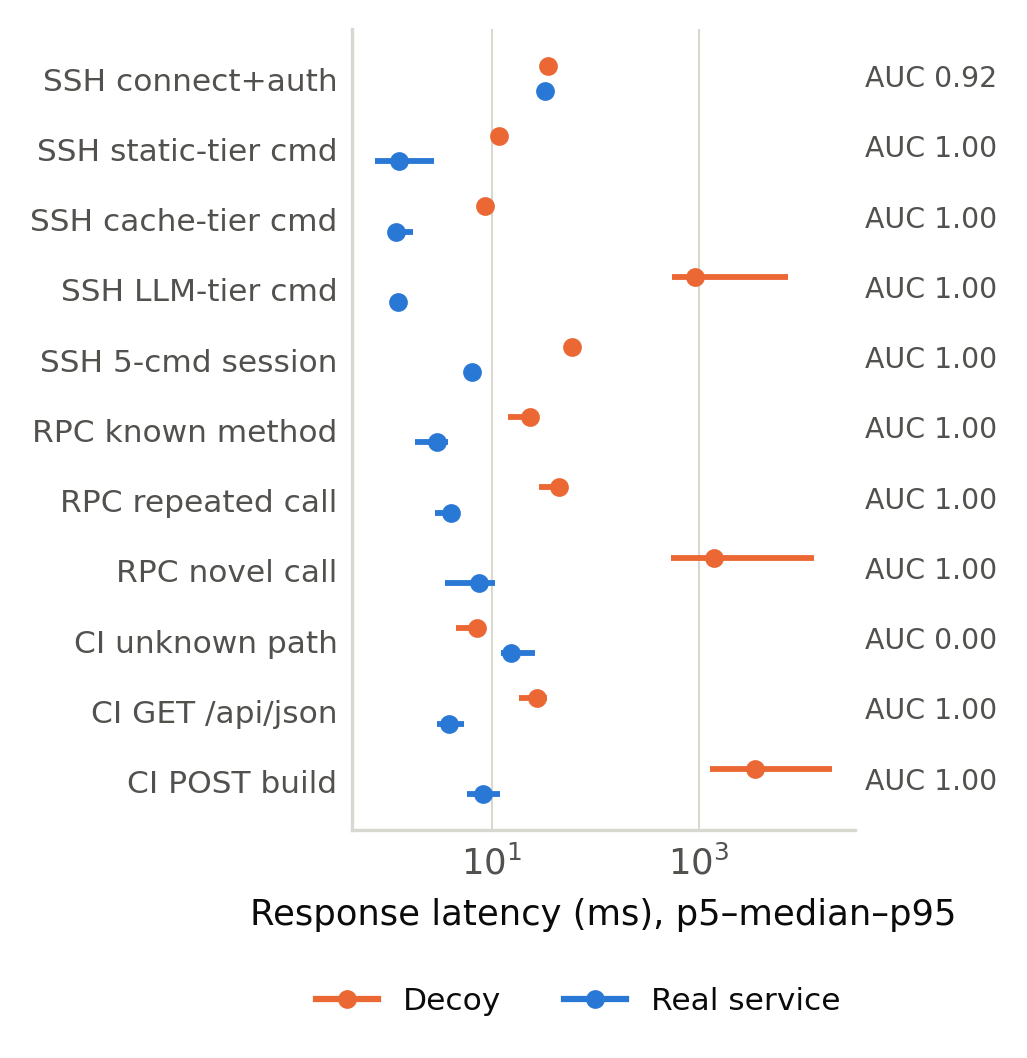
\includegraphics[width=0.95\columnwidth]{figures/fig_latency.png}
\caption{E2: latency of decoy and reference per probe class (p5, median, p95 over 30 trials; logarithmic axis). AUC is the probability that the decoy's reply is slower.}
\label{fig:latency}
\end{figure}

\subsection{Tier exposure over the attack corpus}
\label{sec:res-corpus}
Table~\ref{tab:corpus} and Fig.~\ref{fig:tiers} report E3 for the corpus classes served by each decoy. All 2,500 payloads reached the model: none matched the static table, none hit the cold cache, and no request failed. The static table covers interactive reconnaissance commands, whereas the corpus consists of exploitation strings (URL-encoded command injection, SQL injection, XML external entities, serialized RPC calls), none of which equals a table entry. The model's median latency over the corpus was 1,363\,ms, with a p95 of 8,567\,ms and a maximum of 32,534\,ms; the per-service medians in Table~\ref{tab:corpus} lie between 1,099 and 2,673\,ms, two to three orders of magnitude above the reference services' replies to the same request classes. Every exploitation attempt in the corpus therefore presented the timing signature of Section~\ref{sec:res-time}. On the second pass, 100\% of the sample was served from the warm cache at a median of 3.4\,ms (p95 5.1\,ms), confirming that the cache removes the model's latency whenever it hits. The question is how often it can.

\begin{table}[!t]
\caption{E3: model-tier reply latency over the attack corpus (ms) and the reference service's median for the same request class}
\label{tab:corpus}
\centering
\footnotesize
\renewcommand{\arraystretch}{1.12}
\setlength{\tabcolsep}{4pt}
\begin{tabular}{@{}lrrrrrr@{}}
\toprule
Service & $n$ & to model & median & p95 & max & ref.\ med. \\
\midrule
SSH shell & 1862 & 1862 (100\%) & 1,369 & 8,828 & 32,534 & 1.2 \\
SQL gateway & 474 & 474 (100\%) & 1,439 & 8,039 & 21,550 & -- \\
AI API & 136 & 136 (100\%) & 1,099 & 5,016 & 11,563 & -- \\
JSON-RPC & 18 & 18 (100\%) & 1,192 & 5,330 & 5,330 & 7.6 \\
CI server & 10 & 10 (100\%) & 2,673 & 11,273 & 11,273 & 8.3 \\
\bottomrule
\end{tabular}
\end{table}

\begin{figure}[!t]
\centering
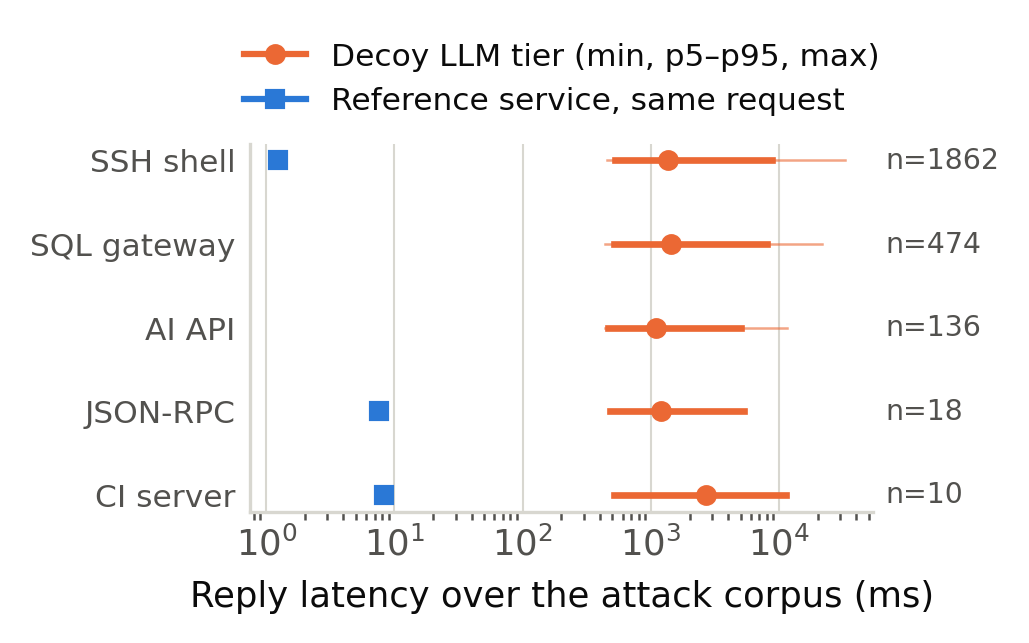
\includegraphics[width=0.95\columnwidth]{figures/fig_tiers.png}
\caption{E3: latency of the model's reply to the attack corpus, per service (median, p5--p95 and min--max, logarithmic axis), against the median reply of the reference service to the same class of request where one exists.}
\label{fig:tiers}
\end{figure}

\subsection{What caching can and cannot hide}
\label{sec:res-cache}
E4 bounds the benefit of a warm cache for traffic the honeypot has not seen. The 2,500 payloads carry 2,500 distinct exact keys and 2,498 distinct normalized keys. Warming the cache with half of the corpus and replaying the other half gives 0 exact-key hits (0\%) and 2 normalized-key hits (0.2\%); Table~\ref{tab:cache} gives the per-service breakdown. Normalization recovers reuse only where attackers repeat a template with different literals. The remainder of the corpus is structurally distinct and reaches the model on first sight, whatever the cache holds.

\begin{table}[!t]
\caption{E4: normalized-key cache hits on the held-out half of the corpus}
\label{tab:cache}
\centering
\footnotesize
\renewcommand{\arraystretch}{1.12}
\begin{tabular}{@{}lrrr@{}}
\toprule
Service & held-out & hits & rate \\
\midrule
AI API & 65 & 0 & 0.0\% \\
CI server & 3 & 0 & 0.0\% \\
SQL gateway & 229 & 2 & 0.9\% \\
SSH shell & 943 & 0 & 0.0\% \\
JSON-RPC & 10 & 0 & 0.0\% \\
\bottomrule
\end{tabular}
\end{table}

\section{Discussion}
\label{sec:discussion}
\subsection{Ranking the mitigations}
The three fingerprint classes differ in what removing them costs. \emph{Identity leaks} (banner, client-version string, \texttt{Server} header, missing \texttt{X-Jenkins} headers) are configuration: \texttt{asyncssh} accepts a custom version string, and the HTTP decoys can set headers copied from the product they imitate. \emph{Protocol-coverage gaps} (\texttt{exec}, batch JSON-RPC, malformed-body handling, \texttt{HEAD} and \texttt{/login}, credential acceptance) require code but no model: each is a deterministic behavior of the reference implementation that can be copied, and rejecting some credentials costs nothing in captured intelligence. \emph{Fast-path semantic errors} are the cheapest of all to fix and the most damaging, because they occur precisely on the commands the static tier exists to answer instantly; arithmetic expansion and compound-command splitting are a few lines. Together these fixes remove every distinguishing probe in Table~\ref{tab:conf}; the decoy's fixed block number did not distinguish it here only because the reference chain was idle, and should advance with time in deployment.

Timing is the hard case. The fast-tier gap could be closed by moving the static table into the decoy process, eliminating the HTTP hop, and by answering the authentication request before logging it. The LLM-tier gap cannot be closed by caching, because Section~\ref{sec:res-cache} shows that new attack traffic almost entirely misses even a normalized cache; it can only be narrowed by making generation faster (a smaller local model, speculative decoding, or streaming the first bytes early) or hidden by making the fast tiers artificially slow so that no reply is ever fast, which imposes the honeypot's worst latency on every command and is itself a fingerprint against a local reference. The phase-adaptive routing of Magazov et al.~\cite{ref11} and the curated-input design of Ragsdale and Boppana~\cite{ref6} are the two published directions consistent with our data: route what can be answered deterministically to a deterministic tier, and send to the model only what must be generated.

\subsection{Limitations}
All measurements are on one machine over loopback, so the fast-tier gaps are laboratory figures that Internet jitter would largely mask; the LLM-tier gap would not be masked. The reference services are one implementation each, and one probe (the unknown-method error code) shows the decoy closer to the JSON-RPC specification~\cite{ref13} than the reference client is; a defender should compare against the exact software being imitated. The LLM tier's latency depends on the hosted provider at the time of measurement. The corpus is the platform's existing evaluation set, so the tier shares describe exploitation traffic and would differ for a corpus of interactive sessions. Two of the five decoys have no reference and were not compared.

\section{Conclusion}
An LLM-backed honeypot can be distinguished from the service it imitates in three ways: by what it reports about itself, by how quickly it replies, and by what its fast path computes incorrectly. Against reference implementations of SSH, Ethereum JSON-RPC and Jenkins, 21 of 28 black-box probes revealed the decoy, the model tier was separable by a single timing observation with AUC 1.000 in every protocol, and 100\% of a real-world attack corpus reached that tier. The identity and protocol gaps are cheap to close and this paper lists them; the timing gap is not closed by caching, which reused 0.2\% of held-out traffic even with normalized keys, and must be addressed by faster generation or by routing more of the traffic away from the model.

\begin{thebibliography}{00}
\bibitem{ref1} N. Provos, ``A virtual honeypot framework,'' in \emph{Proc. 13th USENIX Security Symposium}, San Diego, CA, USA, 2004, pp. 1--14.
\bibitem{ref2} P. Defibaugh-Chavez, R. Veeraghattam, M. Kannappa, S. Mukkamala, and A. H. Sung, ``Network based detection of virtual environments and low interaction honeypots,'' in \emph{Proc. IEEE SMC Information Assurance Workshop}, West Point, NY, USA, 2006, pp. 283--289.
\bibitem{ref3} A. Vetterl and R. Clayton, ``Bitter Harvest: Systematically fingerprinting low- and medium-interaction honeypots at Internet scale,'' in \emph{Proc. 12th USENIX Workshop on Offensive Technologies (WOOT '18)}, Baltimore, MD, USA, 2018.
\bibitem{ref4} S. Morishita, T. Hoizumi, W. Ueno, R. Tanabe, C. Ganan, M. J. G. van Eeten, K. Yoshioka, and T. Matsumoto, ``Detect me if you... oh wait. An Internet-wide view of self-revealing honeypots,'' in \emph{Proc. IFIP/IEEE Symp. Integrated Network and Service Management (IM)}, Washington, DC, USA, 2019, pp. 134--143.
\bibitem{ref5} M. Sladic, V. Valeros, C. Catania, and S. Garcia, ``LLM in the shell: Generative honeypots,'' 2023, \emph{arXiv:2309.00155}.
\bibitem{ref6} J. Ragsdale and R. V. Boppana, ``On designing low-risk honeypots using generative pre-trained transformer models with curated inputs,'' \emph{IEEE Access}, vol. 11, pp. 117528--117545, 2023, doi: 10.1109/ACCESS.2023.3326104.
\bibitem{ref7} S. B. Weber, M. Feger, and M. Pilgermann, ``Don't stop believin': A unified evaluation approach for LLM honeypots,'' \emph{IEEE Access}, vol. 12, 2024, doi: 10.1109/ACCESS.2024.3472460.
\bibitem{ref8} P. Malhotra, ``LLMHoney: A real-time SSH honeypot with large language model-driven dynamic response generation,'' 2025, \emph{arXiv:2509.01463}.
\bibitem{ref9} R. A. Bridges, T. R. Mitchell, M. Munoz, and T. Henriksson, ``SoK: Honeypots \& LLMs, more than the sum of their parts?,'' 2025, \emph{arXiv:2510.25939}.
\bibitem{ref10} R. Magazov, K. Abeshev, Y. Shamuratov, F. Uralova, and G. Aksholak, ``Benchmarking LLM backends for generative SSH honeypots: Security, fidelity, hallucination, latency, and stability,'' \emph{AI}, vol. 7, no. 8, art. 287, 2026, doi: 10.3390/ai7080287.
\bibitem{ref11} R. Magazov, F. Uralova, K. Abeshev, G. Akhmedi, and G. Aksholak, ``Phase-adaptive model routing in LLM-driven SSH honeypots: Balancing response fidelity and latency across the attack lifecycle,'' \emph{Future Internet}, vol. 18, no. 7, art. 359, 2026, doi: 10.3390/fi18070359.
\bibitem{ref12} T. Ylonen and C. Lonvick, ``The Secure Shell (SSH) Transport Layer Protocol,'' IETF RFC 4253, Jan. 2006.
\bibitem{ref13} JSON-RPC Working Group, ``JSON-RPC 2.0 Specification,'' 2013. [Online]. Available: \url{https://www.jsonrpc.org/specification}
\bibitem{ref14} Ethereum Foundation, ``Ethereum JSON-RPC Specification.''. [Online]. Available: \url{https://ethereum.github.io/execution-apis/}
\bibitem{ref15} H. B. Mann and D. R. Whitney, ``On a test of whether one of two random variables is stochastically larger than the other,'' \emph{Annals of Mathematical Statistics}, vol. 18, no. 1, pp. 50--60, 1947.
\bibitem{ref16} Truffle Suite, ``Ganache: A personal Ethereum blockchain for development,'' ConsenSys. [Online]. Available: \url{https://archive.trufflesuite.com/ganache/}
\end{thebibliography}

\end{document}
